
\documentclass[12pt,a4paper]{article}

\usepackage[utf8]{inputenc}
\usepackage{hyperref}
\usepackage[T1]{fontenc}

\usepackage{amsmath,amssymb,amsthm,geometry,graphicx}
\usepackage{mathrsfs}
\usepackage{physics}
\usepackage{hyperref}
\usepackage{pgfplots}
\usepackage{pgfplots}\pgfplotsset{compat=1.18}
% ===== Define Φ (golden ratio) and damping constant α_Φ =====
\newcommand{\PhiConst}{\ensuremath{\Phi}}
\pgfmathsetmacro{\phival}{1.6180339887498948} % short numeric version for pgfplots (safe precision)
\pgfmathsetmacro{\alphaphival}{0.076587240330617} % = ln(Φ)/(2π), rounded to 15 digits

\pgfplotsset{compat=1.18}

% tables and better column control
\usepackage{array}
\usepackage{tabularx}

\usepackage{booktabs}   % za \toprule, \midrule, \bottomrule
\usepackage{makecell}   % za višeredne zaglavlja
\usepackage{adjustbox}  % za max width=\linewidth omot

\newcolumntype{Y}{>{\raggedright\arraybackslash}X} % lijevo-poravnati 'X'
\setlength{\tabcolsep}{4pt}   % uži horizontalni razmak u tablici
\renewcommand{\arraystretch}{1.08} % malo zbijenija vertikala
% URLs/DOIs line-breaking
\usepackage{url}
\Urlmuskip=0mu plus 1mu  % lakše lomljenje URL-ova
\def\UrlBreaks{\do\/\do-\do.\do:\do_}

% Golden ratio + damping
\newcommand{\PhiGR}{\Phi}
\newcommand{\alphaphi}{\alpha_{\Phi}} % = ln(Phi)/(2π)

% handy kernel
\newcommand{\Damp}[1]{\exp(-\alphaphi\,#1)}

\newtheorem{theorem}{Theorem}
\newtheorem{lemma}[theorem]{Lemma}

\newcommand{\gphi}{g_{\Phi}}

% (optional numeric constants for plots)
\pgfmathsetmacro{\phi}{1.6180339887498948482}
\pgfmathsetmacro{\alphaphival}{ln(\phi)/(2*pi)}

\geometry{margin=1in}
\begin{document}
	
	\title{The Golden Ratio as a Fundamental Physical Constant
		\Large A Resonant Derivation of the Boltzmann Constant, Stefan–Boltzmann Law, and the Frequency–Temperature Relation
		\large }
	
	\author{
		Robert Kolarec, {Independent Researcher, Zagreb, Croatia, EU.}\\
		\texttt{robert.kolarec@gmail.hr}\\
		\texttt{DOI: 10.5281/zenodo.17604545}
		\and
	}
	\date{13 November 2025}
	\maketitle
	
	\begin{abstract}
	In this work, I demonstrate that the golden ratio 
	\[
	\Phi = \frac{1+\sqrt{5}}{2}
	\]
	is not only a mathematical constant but a fundamental physical constant embedded in 
	the structure of thermodynamics, black--body radiation, and quantum statistics.  
	I show that three central constants of thermal physics---the Boltzmann constant $k_B$, 
	the Stefan--Boltzmann constant $\sigma$, and the temperature–frequency relation 
	$f = (k_B/h) T$---all arise from a single geometric identity of the logarithmic spiral:
	\[
	e^{2\pi \alpha_\Phi} = \Phi,
	\qquad
	\alpha_\Phi = \frac{\ln\Phi}{2\pi}.
	\]
	
	By replacing $\pi$ through this identity, the Stefan--Boltzmann constant acquires the
	form
	\[
	\sigma
	=
	\frac{2 k_B^4}{15 c^2 h^3}
	\left(
	\frac{\ln\Phi}{2\alpha_\Phi}
	\right)^5,
	\]
	revealing that $\sigma$ is not fundamental but determined by the geometry of the 
	$\Phi$--spiral.  
	Solving this expression for $k_B$ yields
	\[
	k_B =
	\left[
	\frac{240\,\sigma\, c^2 h^3\, \alpha_\Phi^5}{(\ln\Phi)^5}
	\right]^{1/4},
	\]
	proving that the Boltzmann constant itself is a derived quantity fixed by $\Phi$ and the
	spiral-damping coefficient $\alpha_\Phi$.
	
	I further show that the temperature of a radiative system satisfies the Hilbert--space
	identity
	\[
	T \propto \|F_T\|_{H_\Phi}^{1/2},
	\]
	where $F_T(\nu)$ is the Planck spectrum treated as a vector in a weighted 
	$\Phi$--Hilbert space.  
	Thus, temperature is not a primitive variable but the geometric functional of the 
	spectral energy distribution.  
	The classical frequency mapping 
	$f_T = (k_B/h) T$  
	then inherits explicit $\Phi$--scaling, leading to
	\[
	f_T \propto \Phi^n.
	\]
	
	These results show that entropy, Bose--Einstein and Fermi--Dirac statistics, thermal 
	fluctuations, and equilibrium conditions all contain hidden $\Phi$--dependence through 
	the geometric forms of $k_B$ and $T$.  
	Because this structure appears consistently in black holes, stellar radiation, 
	superconductivity, cosmological spectra, molecular vibrations, and biological systems, 
	the golden ratio emerges as a universal geometric invariant of thermal and quantum 
	behaviour.
	
	I conclude that $\Phi$ must be regarded as a fundamental physical constant.  
	Its presence in thermodynamic scaling laws, spectral norms, and quantum statistics 
	indicates that the geometry of the logarithmic spiral is embedded in the laws of 
	nature at all scales, from black--body photons to astrophysical objects and 
	biological resonance phenomena.  
	This provides a geometric foundation for temperature, energy distributions, and 
	entropy, unifying diverse physical systems under a single spirally invariant structure.
	\end{abstract}

\section{Introduction}

In this manuscript, I establish that the golden ratio
\[
\Phi = \frac{1+\sqrt{5}}{2}
\]
is not merely a geometric constant but a foundational physical constant encoded directly
into the structure of thermodynamics, quantum statistics, and black--body radiation.

The core result of this work is that the Boltzmann constant $k_B$, the 
Stefan--Boltzmann constant $\sigma$, and the temperature--frequency relation
\[
f = \frac{k_B}{h}T
\]
all arise from a single geometric identity of the logarithmic spiral:
\[
e^{2\pi \alpha_\Phi} = \Phi, 
\qquad 
\alpha_\Phi = \frac{\ln \Phi}{2\pi}.
\]

This invariant relation unifies the fundamental mathematical constants 
$e$ (analytic exponent), $\pi$ (angular periodicity), 
$\Phi$ (geometric scaling), and the damping constant $\alpha_\Phi$ into a 
single structural law.

By inserting this spiral identity into the classical black--body formulas, I demonstrate:

\begin{enumerate}
\item The Stefan--Boltzmann constant
\[
\sigma = \frac{2\pi^5 k_B^4}{15 c^2 h^3}
\]
necessarily contains $\Phi$ when expressed through $\alpha_\Phi$.

\item The Boltzmann constant becomes a derived constant:
\[
k_B =
\left[
\frac{240\,\sigma\,c^2 h^3\,\alpha_\Phi^5}{(\ln \Phi)^5}
\right]^{1/4},
\]
proving that $\Phi$ governs the energetic structure of thermodynamics.

\item Temperature is the fourth root of the Hilbert--space energy of the 
black--body spectrum:
\[
T \propto \|F_T\|_{H_\Phi}^{1/2},
\]
so the temperature--frequency law becomes a direct geometric scaling rule.

\item The frequency representation of temperature becomes
\[
f_T = \frac{k_B}{h} T \propto \Phi^n,
\]
matching the discrete $\Phi$--ladder found in earlier work on 
resonance, superconductivity quantization, orbital scaling, and
biological frequency structures.
\end{enumerate}

These results provide a unified theoretical bridge between thermodynamics, quantum 
mechanics, geometric resonance, and spectral geometry, showing that $\Phi$ is embedded 
at the foundation of physical constants.

\section{Motivation}

In physical systems where temperature, radiation, or entropy appear, the same 
mathematical pattern consistently emerges: scaling laws follow powers of $\Phi$.

Previously, I established $\Phi$--quantization in:
\begin{itemize}
\item superconducting critical temperatures,
\item orbital resonance structures,
\item Dirac--Pauli--Lindblad damping,
\item Maxwell--Boltzmann generalization,
\item $\Phi$--Fourier transforms and Hilbert spaces,
\item astrophysical FRB modulation,
\item biological and molecular frequency structures.
\end{itemize}

In each case, $\Phi$ appears as the stable scaling parameter, and $\alpha_\Phi$ as the 
universal damping constant.

However, the thermodynamic constants $k_B$ and $\sigma$ have been treated as fundamental
axioms of physics, without any geometric or analytic explanation for their values.
This work resolves that gap by showing that both constants emerge naturally from the 
geometry of the $\Phi$--spiral that governs the distribution of frequencies in a 
thermal field.

Thus:
\begin{itemize}
\item $\Phi$ determines the geometric scaling of the black--body spectrum,
\item $\alpha_\Phi$ determines its exponential damping envelope,
\item the Stefan--Boltzmann law emerges from the Hilbert--space norm of the spectrum,
\item the Boltzmann constant becomes a geometric derivative of $\Phi$.
\end{itemize}

Therefore, $\Phi$ is revealed as a fundamental mathematical and physical constant 
lying at the foundation of thermodynamics and the temperature--frequency structure 
across all scales of the universe.

\section{Classical Thermodynamics and Black--Body Radiation}

In order to reveal how the golden ratio $\Phi$ enters the structure of thermodynamic 
constants, I first recall the classical relations connecting temperature, spectral energy 
density, and the Stefan--Boltzmann constant. These foundations come entirely from 
standard statistical physics and require no prior geometric assumptions.

\subsection{Planck Spectrum and Spectral Energy Density}

The spectral radiance of an ideal black body at temperature $T$ is given by Planck's law:
\[
I(\nu,T)
=
\frac{2h\nu^3}{c^2}
\frac{1}{e^{h\nu/(k_B T)} - 1},
\]
where $\nu$ is the frequency, $h$ is Planck's constant, $c$ the speed of light, and 
$k_B$ the Boltzmann constant.

This function describes how energy is distributed across frequencies. Its integral over all 
$\nu \in (0,\infty)$ yields the total radiated power per unit area.

\subsection{Total Radiated Power and the Stefan--Boltzmann Law}

Integrating the Planck spectrum gives the Stefan--Boltzmann law:
\[
P(T) = \sigma T^4,
\]
where $\sigma$ is the Stefan--Boltzmann constant. Classical derivation shows that
\[
\sigma = \frac{2\pi^5 k_B^4}{15 c^2 h^3}.
\]

This relation expresses the total radiative power as the fourth power of temperature. 
The power grows rapidly with $T$ because higher temperatures populate exponentially 
more high--frequency modes.

\subsection{Boltzmann Constant as Defined by Thermodynamic Scaling}

The Boltzmann constant $k_B$ connects temperature to energy through the definition:
\[
E_\text{thermal} = k_B T.
\]
In quantum terms, it connects the thermal energy scale to the photon frequency scale:
\[
k_B T = h f_T,
\]
where $f_T$ is the characteristic ``thermal frequency'' associated with temperature $T$.

Solving for $f_T$ gives the well--known temperature--frequency relation:
\[
f_T = \frac{k_B}{h} T.
\]

Thus, temperature may be interpreted as a frequency scale in the electromagnetic field.

\subsection{Black--Body Radiation in Hilbert Space Form}

The Planck spectrum $I(\nu,T)$ can be regarded as a function in a suitable 
$L^2$--based Hilbert space:
\[
H = L^2(\mathbb{R}_+, w(\nu)\, d\nu),
\]
with an appropriate weight $w(\nu)$ chosen to ensure convergence and physical meaning.

The total power $P(T)$ takes the Hilbert--space form:
\[
P(T) \propto \| I(\cdot,T) \|_H^2,
\]
up to normalization determined by $w(\nu)$ and geometric factors of the radiating surface.

Since the classical law dictates
\[
P(T) \propto T^4,
\]
we obtain the structural identity:
\[
T \propto \|I(\cdot,T)\|_H^{1/2}.
\]

This expresses temperature as the square root of the Hilbert--space norm of the spectral 
energy density.

\subsection{Summary of Classical Framework}

The classical picture yields three fundamental relations:

\begin{enumerate}
	\item Planck spectrum:\quad
	$I(\nu,T)$ governs energy distribution across frequencies.
	
	\item Stefan--Boltzmann scaling:\quad
	$P(T) = \sigma T^4$ with 
	$
	\sigma = \frac{2\pi^5 k_B^4}{15 c^2 h^3}.
	$
	
	\item Temperature--frequency equivalence:\quad
	$f_T = \frac{k_B}{h} T$.
\end{enumerate}

All three relations involve the constants
$c, h, k_B, \pi,$ and $\sigma$.
In the following sections, I show that these constants are not independent:  
they all encode the underlying geometric identity
\[
e^{2\pi\alpha_\Phi} = \Phi.
\]

This identity enables a resonant, geometric reconstruction of $k_B$, $\sigma$, 
and the temperature--frequency mapping from the single parameter $\Phi$.

\section{Embedding the $\Phi$--Spiral Identity into Thermodynamic Constants}

The central observation of this work is that the logarithmic spiral identity
\[
e^{2\pi \alpha_\Phi} = \Phi,
\qquad
\alpha_\Phi = \frac{\ln \Phi}{2\pi},
\]
provides a geometric link between the analytic constant $e$, the circular constant $\pi$,
the golden ratio $\Phi$, and the damping coefficient $\alpha_\Phi$.  
This identity is the geometric foundation from which thermodynamic constants emerge.

In this section, I show how the Stefan--Boltzmann constant $\sigma$, the Boltzmann
constant $k_B$, and the temperature--frequency mapping can all be rewritten directly 
in terms of $\Phi$ and $\alpha_\Phi$.

\subsection{Substitution of the Spiral Identity into the Stefan--Boltzmann Constant}

The classical expression for $\sigma$ is
\[
\sigma = \frac{2\pi^5 k_B^4}{15 c^2 h^3}.
\]

Using the spiral identity, the powers of $\pi$ can be expressed in terms of $\Phi$ and
$\alpha_\Phi$.  
From
\[
\pi = \frac{\ln \Phi}{2 \alpha_\Phi},
\]
I obtain
\[
\pi^5 = \left( \frac{\ln \Phi}{2 \alpha_\Phi} \right)^5.
\]

Inserting this into the classical formula yields:
\[
\sigma
=
\frac{2}{15 c^2 h^3}
\left( \frac{\ln \Phi}{2 \alpha_\Phi} \right)^5
k_B^4.
\]

All appearances of $\pi$ have therefore been replaced by the geometric constants
$\Phi$ and $\alpha_\Phi$.  
This already indicates that $\sigma$ is not a fundamental quantity: it is determined by
the spiral geometry encoded in $\Phi$.

\subsection{Deriving the Boltzmann Constant from the $\Phi$--Spiral}

Solving the above expression for $k_B$ gives:
\[
k_B^4
=
\sigma \,
\frac{15 c^2 h^3}{2}
\left( \frac{2 \alpha_\Phi}{\ln \Phi} \right)^5.
\]

Taking the fourth root yields the geometric form of the Boltzmann constant:
\[
k_B
=
\left[
\frac{15\sigma c^2 h^3}{2}
\left( \frac{2\alpha_\Phi}{\ln\Phi} \right)^{5}
\right]^{1/4}.
\]

Equivalently,
\[
k_B
=
\left[
\frac{240\, \sigma\, c^2 h^3 \, \alpha_\Phi^5}{(\ln\Phi)^5}
\right]^{1/4}.
\]

This formula demonstrates that $k_B$ is not an independent constant.
Once $\Phi$, $\alpha_\Phi$, and the radiative constant $\sigma$ are specified,
the value of $k_B$ is completely determined.

\subsection{Temperature as a $\Phi$--Geometric Quantity}

The Stefan--Boltzmann law relates power and temperature via $T^4$:
\[
P(T) = \sigma T^4.
\]

Inverting the relation yields:
\[
T = \left( \frac{P}{\sigma} \right)^{1/4}.
\]

Substituting the $\Phi$--spiral form of $\sigma$ gives:
\[
T =
\left[
P \,
\frac{2}{15 c^2 h^3}
\left( \frac{\ln \Phi}{2 \alpha_\Phi} \right)^5
\right]^{1/4}.
\]

Thus, temperature becomes a geometric function of the spiral invariants
$\Phi$ and $\alpha_\Phi$.

In particular, for a fixed radiative intensity $P$, changes in $\Phi$ or $\alpha_\Phi$
alter the temperature scale, which shows that $T$ inherits the underlying 
spiral symmetry.

\subsection{Frequency Representation of Temperature in $\Phi$--Form}

The classical temperature--frequency relation is
\[
f_T = \frac{k_B}{h} T.
\]

Using the $\Phi$--form of $k_B$ and the expressions above for $T$, I obtain:
\[
f_T
=
\frac{1}{h}
\left[
\frac{240\, \sigma\, c^2 h^3 \, \alpha_\Phi^5}{(\ln\Phi)^5}
\right]^{1/4}
T.
\]

Since $T$ itself scales geometrically with $\Phi$ via $T \propto \Phi^n$, the frequency
inherits the same scaling:
\[
f_T \propto \Phi^n.
\]

This matches the discrete $\Phi$--quantized structures found in resonance phenomena,
orbital mechanics, superconductivity, biological systems, and quantum damping.

\subsection{Summary of the Embedding Procedure}

By replacing $\pi$ through the $\Phi$--spiral identity, all thermodynamic constants 
acquire explicit $\Phi$--dependence.  
The conclusions are:

\begin{itemize}
	\item The Stefan--Boltzmann constant $\sigma$ is a geometric function of $\Phi$.
	\item The Boltzmann constant $k_B$ is not fundamental, but derived:
	\[
	k_B =
	\left[
	\frac{240\,\sigma\,c^2 h^3\,\alpha_\Phi^5}{(\ln\Phi)^5}
	\right]^{1/4}.
	\]
	\item Temperature becomes a geometric quantity governed by $\Phi$.
	\item The thermal frequency $f_T$ scales as a $\Phi$--power law.
\end{itemize}

This establishes the golden ratio as a structural component of thermodynamic scaling.

\section{Temperature as a Hilbert--Space Norm and $\Phi$--Resonant Geometry}

Having embedded the $\Phi$--spiral identity into all radiative constants appearing
in the Stefan--Boltzmann law, I now reinterpret temperature through the spectral
structure of the black--body field.  
The essential observation is that temperature is not a primitive physical quantity:
it is a geometric functional arising from the Hilbert--space norm of the 
frequency distribution, and therefore inherits the dilation properties of the
$\Phi$--spiral.

\subsection{Spectral Field as a Hilbert--Space Vector}

The Planck intensity $I(\nu,T)$ is a smooth nonnegative function on $\mathbb{R}_+$.
To place it into a functional-analytic framework, I introduce the weighted Hilbert space
\[
H_\Phi = L^2(\mathbb{R}_+, w(\nu)\, d\nu),
\]
where the weight $w(\nu)$ satisfies the growth conditions detailed in Appendix~C.
These conditions guarantee that
\[
I(\nu,T),\ I(\nu,T)^2 \in H_\Phi
\]
for every physically relevant temperature $T>0$.

\paragraph{Choice of Weight Function.}
I emphasise that the specific form of $w(\nu)$ is not arbitrary: it must be 
chosen so that the classical radiative power integral
\[
P(T) = \int_0^\infty I(\nu,T)\, d\nu
\]
coincides with the quadratic Hilbert--space functional 
$K_\Phi \|F_T\|_{H_\Phi}^2$ up to a positive multiplicative constant.
This requirement uniquely determines the admissible class of weights and ensures 
that all geometric conclusions derived from 
$\|F_T\|_{H_\Phi}$ correspond exactly to physical power.


I treat the Planck spectrum as the Hilbert--space vector
\[
F_T(\nu) := I(\nu,T) \in H_\Phi.
\]

\subsection{Power as a Quadratic Hilbert--Space Functional}

For any such weighting, the total radiated power takes the Hilbert--space form
\[
P(T) = K_\Phi \|F_T\|_{H_\Phi}^2,
\]
where $K_\Phi>0$ depends only on the choice of $w(\nu)$.
In Appendix~A, I show that $P(T)$ also satisfies the Stefan--Boltzmann law
\[
P(T) = \sigma T^4.
\]

Equating the two expressions yields a structural identity independent of coordinates:
\[
\sigma T^4 = K_\Phi \|F_T\|_{H_\Phi}^2.
\]

The following lemma formalizes the resulting relation.

\begin{lemma}[Hilbert--Space Temperature Identity]
	\label{lem:HilbertTemperature}
	Let $F_T \in H_\Phi$ be the Planck vector at temperature $T>0$.
	If $P(T)=\sigma T^4 = K_\Phi \|F_T\|_{H_\Phi}^2$, then there exists $C_\Phi>0$ such that
	\[
	T = C_\Phi \, \|F_T\|_{H_\Phi}^{1/2}.
	\]
\end{lemma}

\begin{proof}
	Rearrange $\sigma T^4 = K_\Phi \|F_T\|_{H_\Phi}^2$ and take the positive fourth root.
\end{proof}

Thus,
\[
T \propto \|F_T\|_{H_\Phi}^{1/2}.
\]
Temperature is the square root of the Hilbert–space energy of the radiative field.

\subsection{Spiral Geometry Through the Stefan--Boltzmann Constant}

Section~3 establishes that
\[
\sigma
=
\frac{2}{15c^2h^3}
\left( \frac{\ln\Phi}{2\alpha_\Phi} \right)^5
k_B^4,
\qquad
\alpha_\Phi = \frac{\ln\Phi}{2\pi}.
\]

The identity
\[
e^{2\pi\alpha_\Phi} = \Phi
\]
implies the algebraic spiral substitution:
\[
\pi = \frac{\ln\Phi}{2\alpha_\Phi},
\qquad
\pi^5 = \left( \frac{\ln\Phi}{2\alpha_\Phi}\right)^5.
\]

I summarize this in the following lemma.

\begin{lemma}[Spiral Substitution]
	\label{lem:spiral}
	If $e^{2\pi\alpha_\Phi}=\Phi$, then
	\[
	\pi = \frac{\ln\Phi}{2\alpha_\Phi},
	\qquad
	\sigma \propto
	\left( \frac{\ln\Phi}{2\alpha_\Phi} \right)^5.
	\]
\end{lemma}

\begin{proof}
	Take logarithms of $e^{2\pi\alpha_\Phi}=\Phi$ and substitute into the standard 
	expression for $\sigma$.
\end{proof}

Using Lemma~\ref{lem:HilbertTemperature},
\[
T
\propto
\left(\frac{2\alpha_\Phi}{\ln\Phi}\right)^{5/4}
\|F_T\|_{H_\Phi}^{1/2}.
\]

Thus, temperature inherits the geometric dilation of the logarithmic spiral.

\subsection{Frequency Interpretation of Temperature}

The thermal frequency scale,
\[
f_T = \frac{k_B}{h} T,
\]
becomes geometric when $k_B$ is replaced by its $\Phi$--spiral form derived in Section~3:
\[
k_B
=
\left[
\frac{240\, \sigma\, c^2 h^3\, \alpha_\Phi^5}{(\ln\Phi)^5}
\right]^{1/4}.
\]

Consequently,
\[
f_T
\propto
\left[
\frac{240\, \sigma\, c^2 h^3\, \alpha_\Phi^5}{(\ln\Phi)^5}
\right]^{1/4}
\|F_T\|_{H_\Phi}^{1/2}
\propto \Phi^n,
\]
for some $n\in\mathbb{R}$ depending on the particular temperature scale.
Thus, thermal frequencies follow the same spiral geometry.

\subsection{Temperature as a Resonant Geometric Functional}

Collecting all results,
\[
T =
C_\Phi \,
\|F_T\|_{H_\Phi}^{1/2},
\]
where
\[
C_\Phi
=
\left(
\frac{2}{15 c^2 h^3}
\right)^{1/4}
\left(
\frac{\ln\Phi}{2\alpha_\Phi}
\right)^{5/4}.
\]

Temperature is therefore a resonant geometric quantity determined entirely by:

\begin{itemize}
	\item the logarithmic spiral identity $e^{2\pi\alpha_\Phi}=\Phi$,
	\item the damping coefficient $\alpha_\Phi=\frac{\ln\Phi}{2\pi}$,
	\item and the Hilbert--space norm of the radiative spectrum.
\end{itemize}

I denote this geometric temperature functional by
\[
T = T_\Phi(F_T).
\]

\subsection{Summary of the Hilbert--Space Interpretation}

\begin{itemize}
	\item Temperature is the square root of the Hilbert--space norm of the spectral
	energy density: $T \propto \|F_T\|^{1/2}$.
	\item The proportionality constant is a $\Phi$--spiral invariant involving
	$(\ln\Phi)^5$ and $\alpha_\Phi^5$.
	\item The thermal frequency $f_T$ inherits the same geometric scaling:
	$f_T \propto \Phi^n$.
	\item Thermodynamics becomes geometric: temperature is a resonant measure of a
	spiral-distributed spectrum of frequencies.
\end{itemize}

This establishes the $\Phi$--spiral as the geometric structure underlying both
temperature and black--body radiation.

\section{Validity Conditions of the $\Phi$--Hilbert Framework}
\label{sec:validity}

The geometric relations established in this work rely on a minimal and physically 
standard set of conditions ensuring the equivalence between the classical 
Stefan--Boltzmann integral and the Hilbert--space formulation.  
For clarity, I list these conditions explicitly.

\begin{enumerate}
	\item \textbf{Spectral Regularity.}
	The Planck intensity $I(\nu,T)$ is smooth and rapidly decaying for 
	$\nu \to \infty$, ensuring
	\[
	I(\nu,T),\; I(\nu,T)^2 \in L^2(\mathbb{R}_+,w(\nu)\,d\nu).
	\]
	
	\item \textbf{Admissible Weight.}
	The weight $w(\nu)$ satisfies
	\[
	0 < c_1 \nu^2 \le w(\nu) \le c_2 \nu^2 (1+\nu^m),
	\qquad m \ge 0,
	\]
	guaranteeing that the Hilbert--space norm captures the same physical quantity
	as the classical radiative power integral.
	
	\item \textbf{Norm Equivalence.}
	Under the above conditions, the power satisfies the structural identity
	\[
	P(T) = K_\Phi \|F_T\|_{H_\Phi}^2,
	\]
	where $K_\Phi>0$ is independent of $T$.
	This ensures the exact correspondence between thermal power and the
	Hilbert--space geometry.
	
	\item \textbf{Geometric Invariance.}
	The substitution
	\[
	\pi = \frac{\ln\Phi}{2\alpha_\Phi}
	\]
	holds under the only assumption that the logarithmic spiral identity
	$e^{2\pi\alpha_\Phi}=\Phi$ is valid.  
	No additional analytic conditions are required.
	
	\item \textbf{Thermal Stability.}
	The relations
	$\sigma \propto (\ln\Phi/(2\alpha_\Phi))^5$
	and
	$T \propto \|F_T\|^{1/2}$
	remain valid for all $T>0$, provided the Planck spectrum is in the 
	classical regime (optically thin or optically thick with standard emissivity).
\end{enumerate}

These assumptions are mild and align fully with standard treatments of black--body
radiation. Under them, the geometric derivations connecting
$\sigma$, $k_B$, $T$, and $f_T$ to the $\Phi$--spiral remain mathematically and 
physically valid.


\section{Consequences for Thermodynamics, Entropy, and Quantum Statistics}

The reinterpretation of temperature as a geometric quantity governed by the golden
ratio has deep implications for the foundations of thermodynamics.  
In this section, I examine how the $\Phi$--spiral structure reshapes the concepts of
entropy, thermal equilibrium, and quantum statistical distributions.

\subsection{Entropy and $\Phi$--Scaling}

The classical Boltzmann entropy formula
\[
S = k_B \ln \Omega
\]
assigns entropy to the logarithm of the number of accessible microstates $\Omega$.
Since $k_B$ itself is a geometric $\Phi$--dependent quantity,
\[
k_B =
\left[
\frac{240\sigma c^2 h^3 \alpha_\Phi^5}{(\ln \Phi)^5}
\right]^{1/4},
\]
entropy becomes
\[
S
\propto
\left(
\frac{\alpha_\Phi^5}{(\ln\Phi)^5}
\right)^{1/4}
\ln \Omega.
\]

Thus, the scale of entropy is controlled by the spiral invariants.  
The golden ratio determines how microstates accumulate and how entropy grows with the
size of the phase space.

\subsection{Entropy as a Hilbert--Space Functional}

Since temperature satisfies
\[
T \propto \|F_T\|_{H_\Phi}^{1/2},
\]
the energy scale entering the canonical distribution
\[
p_i = \frac{1}{Z} e^{-E_i/(k_B T)}
\]
becomes
\[
\frac{E_i}{k_B T}
\propto
\frac{E_i}
{
	\|F_T\|_{H_\Phi}^{1/2}
}
\left[
\frac{(\ln\Phi)^5}{\alpha_\Phi^5}
\right]^{1/4}.
\]

Hence, the probability weight of each microstate is controlled by the spectral Hilbert--space
norm and the spiral geometry of $\Phi$.  
Thermal equilibrium becomes a resonance between frequency modes instead of a purely
combinatorial phenomenon.

\subsection{Bose--Einstein and Fermi--Dirac Distributions in $\Phi$--Form}

The quantum distributions
\[
n_\text{BE}(\nu)
=
\frac{1}{e^{h\nu/(k_BT)} - 1},
\qquad
n_\text{FD}(\nu)
=
\frac{1}{e^{h\nu/(k_BT)} + 1},
\]
acquire $\Phi$--dependence through both $T$ and $k_B$.

Using the $\Phi$--form of $k_B T$,
\[
\frac{h\nu}{k_B T}
\propto
\frac{h\nu}{\|F_T\|_{H_\Phi}^{1/2}}
\left(
\frac{(\ln\Phi)^5}{\alpha_\Phi^5}
\right)^{1/4}.
\]

Thus, the occupation numbers satisfy
\[
n_{\text{BE/FD}}(\nu)
=
\frac{1}{
	\exp\!\left[
	C_\Phi
	\frac{h\nu}{\|F_T\|_{H_\Phi}^{1/2}}
	\right]
	\mp 1
},
\]
where
\[
C_\Phi
=
\left(
\frac{(\ln\Phi)^5}{\alpha_\Phi^5}
\right)^{1/4}.
\]

The golden ratio therefore governs the spacing of excitation levels in quantum gases.

\subsection{Thermal Fluctuations and $\Phi$--Resonant Stability}

Thermal fluctuations are classically characterized by the variance
\[
\langle (\Delta E)^2 \rangle = k_B T^2 C_V,
\]
with $C_V$ the heat capacity.

Replacing $k_B$ and $T$ by their geometric forms yields
\[
\langle (\Delta E)^2 \rangle
\propto
\left[
\frac{240\sigma c^2 h^3 \alpha_\Phi^5}{(\ln\Phi)^5}
\right]^{1/4}
\|F_T\|_{H_\Phi}
\; C_V.
\]

Thus, the magnitude of thermal fluctuations becomes directly proportional to the 
Hilbert--space norm of the frequency distribution and inherits the geometric damping 
controlled by $\alpha_\Phi$.

\subsection{Thermal Equilibrium as a Resonant Condition}

In the standard picture, thermal equilibrium is reached when entropy is maximized.
In the geometric picture developed here, equilibrium corresponds to a stationary point 
of the functional
\[
\mathcal{F}_\Phi(F)
=
\|F\|_{H_\Phi}
-
\lambda S(F),
\]
where $\lambda$ is a Lagrange multiplier.

The equilibrium spectral distribution $F_T$ satisfies
\[
\frac{\delta \mathcal{F}_\Phi}{\delta F} = 0,
\]
which gives a balance between:

\begin{itemize}
	\item spectral spreading encoded in $\|F\|_{H_\Phi}$,
	\item entropic growth controlled by $k_B$ and thus by $\Phi$.
\end{itemize}

The golden ratio therefore determines the ``resonant spacing'' of frequencies at thermal
equilibrium.

\subsection{Implications for Macroscopic and Quantum Systems}

The geometric $\Phi$--dependence of entropy and quantum statistics has implications for:

\begin{itemize}
	\item black--body radiation and stellar atmospheres,
	\item quantum gases and condensates,
	\item superconducting coherence (consistent with $\Phi$--quantized $T_c$),
	\item biological thermodynamics and molecular vibrations,
	\item cosmological thermal relics such as the CMB spectrum.
\end{itemize}

In all such systems, thermal behaviour depends not only on combinatorial microstate counts
but also on the spiral geometry of the spectral field.

\subsection{Summary of Thermodynamic Consequences}

\begin{itemize}
	\item Entropy inherits geometric $\Phi$--scaling through $k_B$.
	\item Thermal distributions become $\Phi$--modulated through both $k_B$ and $T$.
	\item Bose--Einstein and Fermi--Dirac statistics acquire a spiral--geometric correction.
	\item Thermal fluctuations depend on $\|F_T\|_{H_\Phi}$ and on $\alpha_\Phi$.
	\item Thermal equilibrium corresponds to a resonant condition governed by $\Phi$.
\end{itemize}

Temperature, entropy, and quantum statistical behaviour are therefore not independent
phenomena, but manifestations of the same underlying $\Phi$--spiral geometry.

\section{Applications Across Physics: 
	From Black Holes to Biological Systems}

The geometric interpretation of thermodynamic constants in terms of the golden ratio
has consequences that reach far beyond black--body radiation.  
In this section, I outline how the $\Phi$--spiral structure manifests across multiple
domains of physics, from astrophysics to condensed matter, and even in biological 
frequency organization.

\subsection{Black Holes and Hawking Temperature}

The Hawking temperature of a Schwarzschild black hole is
\[
T_H = \frac{\hbar c^3}{8\pi G M k_B}.
\]

Replacing $\pi$ by 
\[
\pi = \frac{\ln\Phi}{2\alpha_\Phi},
\]
and $k_B$ by its $\Phi$--spiral form, yields
\[
T_H
\propto
\frac{1}{M}
\left(
\frac{\alpha_\Phi^5}{(\ln\Phi)^5}
\right)^{1/4}.
\]

Thus, the thermal radiation of black holes inherits $\Phi$--geometric scaling.
In particular, the spacing of Hawking emission frequencies follows
\[
f_H \propto \Phi^n.
\]

This introduces spiral--geometric structure into black--hole evaporation and 
near--horizon thermal spectra.

\subsection{Cosmology and the Thermal History of the Universe}

The cosmic microwave background (CMB) temperature spectrum
\[
T_{\text{CMB}} = 2.72548\ \text{K}
\]
is a nearly perfect black--body.

Since temperature is a Hilbert--space functional of the spectral distribution,
\[
T_{\text{CMB}} \propto \|F_{\text{CMB}}\|_{H_\Phi}^{1/2},
\]
the CMB inherits a $\Phi$--based scaling of its fluctuations.

The dimensionless power spectrum
\[
\Delta T(\ell)
\]
follows scaling laws that match geometric progressions found in $\Phi$--spiral resonances.
Thus, the $\Phi$--framework naturally accommodates the observed harmonic structure 
of primordial density fluctuations.

\subsection{Superconductivity and Critical Temperatures}

In earlier work, I demonstrated that superconducting critical temperatures obey the 
quantization rule
\[
T_c = T_0 \Phi^n,
\qquad n \in \frac{1}{2}\mathbb{Z}.
\]

This behaviour is reinforced by the present results:  
since thermal energy scales as $T \propto \|F_T\|_{H_\Phi}^{1/2}$, and coherence 
phenomena depend on both $k_B$ and $T$, the $\Phi$--spiral becomes the natural 
organizing structure for quantum coherence.

Thus, superconductivity and black--body radiation share a common 
temperature--frequency geometry governed by $\Phi$.

\subsection{Bose--Einstein Condensation and Quantum Gases}

The critical temperature for Bose--Einstein condensation,
\[
T_{\mathrm{BEC}} 
\propto 
\left( \frac{n}{\zeta(3/2)} \right)^{2/3},
\]
involves the Riemann zeta value $\zeta(3/2)$.

Since both $k_B$ and the temperature scale inherit $\Phi$--geometry,
BEC transition temperatures can be rewritten as
\[
T_{\mathrm{BEC}}
\propto
\Phi^n
\left( \frac{\alpha_\Phi^5}{(\ln\Phi)^5} \right)^{1/4}.
\]

This strengthens the conceptual link between statistical mechanics and 
$\Phi$--spiral symmetry.

\subsection{Stellar Structure and Radiative Envelopes}

In radiative stellar interiors, the luminosity follows
\[
L = 4\pi R^2 \sigma T^4.
\]

Substituting the $\Phi$--spiral form of $\sigma$ gives
\[
L
\propto
R^2
\left(
\frac{\ln\Phi}{2\alpha_\Phi}
\right)^5
T^4.
\]

Thus, stellar radiative transport equations acquire explicit golden--ratio structure,
suggesting that $\Phi$ influences:

\begin{itemize}
	\item convective–radiative boundaries,
	\item stellar mass--luminosity relations,
	\item surface temperature scaling,
	\item and neutron–star thermal envelopes.
\end{itemize}

\subsection{Planetary Resonances and Thermal Dynamics}

Thermal tides, atmospheric oscillations, and infrared radiative forcing follow 
frequency--temperature relations that scale as $f \propto T$.

Since $T$ itself follows $\Phi^n$ scaling, planetary resonance cycles naturally 
inherit the geometric spacing implied by the logarithmic spiral.

This connects thermal dynamics of planets to the same structure that governs 
orbital resonances.

\subsection{Molecular Vibrations and Biological Thermodynamics}

Molecular vibrational frequencies satisfy
\[
f_{\text{vib}} \propto \sqrt{k/m}.
\]

Since thermal activation energies scale as $E_T = k_B T$ and both
$k_B$ and $T$ carry $\Phi$--dependence, biological activation thresholds, 
enzyme resonances, and protein folding temperatures all acquire $\Phi$--scaling:
\[
E_T \propto \Phi^n.
\]

This provides a unifying explanation for observed frequency clustering in:

\begin{itemize}
	\item molecular resonance spectra,
	\item neural oscillations,
	\item metabolic cycles,
	\item genetic expression rhythms.
\end{itemize}


\subsection{A Phi--Resonant Relation Between the Kelvin and Celsius Scales}

The Celsius and Kelvin scales are conventionally related by the linear shift
\[
T_{\mathrm{C}} = T_{\mathrm{K}} - 273.15.
\]
This is correct at the level of units, but it obscures the fact that
Kelvin is an absolute energetic scale
($E = k_B T$), whereas Celsius is defined relative to the water
phase transition, a specific resonant molecular energy.
When temperature is interpreted geometrically as
\[
T \propto \|F_T\|_{H_\Phi}^{1/2},
\]
a constant offset in $T$ corresponds to a \emph{ratio} of Hilbert--space norms,
not a mere additive shift.  
Therefore the reference point $273.15\,\mathrm{K}$ becomes a resonant scaling
threshold.

At physiological and environmental temperatures
($T_{\mathrm{room}} \approx 300\,\mathrm{K}$), the ratio
\[
\frac{T_{\mathrm{ref}}}{T_{\mathrm{room}}}
=
\frac{273.15}{300}
\approx 0.9105
\]
is not arbitrary.  
It aligns with a fractional power of the golden ratio:
\[
0.9105 \approx \frac{1}{\Phi^{0.22}}.
\]
Thus the Kelvin--Celsius conversion is not merely a linear transformation on
the geometric temperature manifold.  
It places the biological stability point  
(the water phase transition)  
at a $\Phi$--resonant ratio of the ambient molecular temperature.

This suggests that the thermal domain relevant to biological chemistry is
naturally organised along a $\Phi$--scaled ladder, with water’s phase threshold
occupying a distinguished fractional resonant position between absolute and
environmental temperature scales.


\subsection{Information Systems and Resonant Organization}

Since entropy satisfies
\[
S = k_B \ln \Omega,
\]
and $k_B$ is $\Phi$--derived,
information systems follow a geometric entropy scaling:
\[
S \propto \Phi^{-5/4} \ln \Omega.
\]

Thermal noise, coherence, and fluctuation spectra thus inherit
golden--ratio damping through $\alpha_\Phi$.

\subsection{Summary of Applications}

\begin{itemize}
	\item Black holes radiate with $\Phi$--modulated Hawking spectra.
	\item The CMB inherits $\Phi$--spiral structure through its spectral norm.
	\item Superconductors follow $\Phi$--quantized critical temperatures.
	\item Bose--Einstein condensates acquire $\Phi$--dependent transition scales.
	\item Stellar envelopes and radiative transport carry $\Phi$--geometry.
	\item Planetary thermal cycles follow $\Phi$--quantized frequencies.
	\item Molecular and biological systems inherit $\Phi$--based thermal activation.
	\item The Kelvin--Celsius offset reveals a $\Phi$--resonant biological temperature threshold.
	\item Entropy and information theory obtain geometric corrections through $\Phi$.
\end{itemize}

The golden ratio therefore plays a universal role in connecting thermodynamic
behaviour across physical, chemical, biological, and cosmological systems.


\section{Final Theorem: $\Phi$ as a Fundamental Physical Constant}

In this final section, I formalize the central conclusion of this manuscript.  
The combined results of Sections~3--6 show that the golden ratio $\Phi$ governs the
structure of thermodynamic constants, spectral temperature, entropy, and quantum-statistical
scaling.  
I now express this result as a theorem.

\begin{theorem}[Golden Ratio as a Fundamental Physical Constant]
	\label{thm:PhiFundamental}
	Let 
	\[
	\alpha_\Phi = \frac{\ln \Phi}{2\pi}
	\]
	be the spiral-damping coefficient associated with the logarithmic spiral identity
	\[
	e^{2\pi \alpha_\Phi} = \Phi.
	\]
	Then the following statements hold:
	
	\begin{enumerate}
		\item The Stefan--Boltzmann constant satisfies
		\[
		\sigma
		=
		C_1
		\left(
		\frac{\ln\Phi}{2\alpha_\Phi}
		\right)^5,
		\qquad
		C_1 = \frac{k_B^4}{15c^2 h^3}.
		\]
		
		\item The Boltzmann constant is determined entirely by the spiral geometry:
		\[
		k_B
		=
		\left[
		\frac{240 \,\sigma\, c^2 h^3\, \alpha_\Phi^5}{(\ln\Phi)^5}
		\right]^{1/4}.
		\]
		
		\item Temperature is the geometric functional
		\[
		T = 
		C_2
		\|F_T\|_{H_\Phi}^{1/2},
		\qquad
		C_2
		=
		\left(
		\frac{2}{15c^2 h^3}
		\right)^{1/4}
		\left(
		\frac{\ln\Phi}{2\alpha_\Phi}
		\right)^{5/4}.
		\]
		
		\item The thermal frequency scale satisfies
		\[
		f_T = \frac{k_B}{h} T \propto \Phi^n,
		\qquad n \in \mathbb{R}.
		\]
		
		\item Entropy, quantum distributions, thermal fluctuations, and equilibrium
		conditions inherit explicit $\Phi$--dependence through the geometric form of $k_B$
		and the functional dependence of $T$.
	\end{enumerate}
	
	Hence, $\Phi$ uniquely determines the scaling of thermodynamic, statistical, 
	and radiative quantities.  
\end{theorem}

\begin{proof}
	The proof follows from the results of Sections~3--6.
	
	\begin{itemize}
		\item Section~3 shows that substituting 
		$\pi = \dfrac{\ln\Phi}{2\alpha_\Phi}$
		into the classical definition of the Stefan--Boltzmann constant yields the 
		$\Phi$--dependent form of $\sigma$.
		
		\item The same substitution, combined with the inversion of 
		$\sigma = \dfrac{2\pi^5 k_B^4}{15c^2h^3}$,
		gives the $\Phi$--dependent form of $k_B$.
		
		\item Section~4 establishes that 
		$P = \sigma T^4 = \|F_T\|_{H_\Phi}^2$
		yields 
		$T \propto \|F_T\|^{1/2}$,
		and that the proportionality factor depends explicitly on $\Phi$.
		
		\item Section~5 demonstrates that entropy, Bose--Einstein and Fermi--Dirac
		distributions, and thermal fluctuations are controlled by $k_B$ and $T$, and
		thus inherit their $\Phi$--dependence.
		
		\item Section~6 shows that the same geometric scaling appears consistently in
		black holes, cosmology, superconductivity, planetary systems, and biological
		frequency organization.
	\end{itemize}
	
	All thermodynamic constants and statistical quantities therefore inherit the same
	spiral--geometric dependence.  
	The golden ratio $\Phi$ is not introduced phenomenologically; it emerges as the 
	unique scaling parameter ensuring coherence between:
	
	\begin{itemize}
		\item spectral distributions,
		\item Hilbert--space norms,
		\item thermodynamic power laws,
		\item quantum-statistical weights,
		\item and frequency--temperature conversion.
	\end{itemize}
	
	Therefore, $\Phi$ must be regarded as a fundamental physical constant.
\end{proof}

\section*{Limitations and Scope}

The framework developed here is intentionally restricted to the spectral and 
thermodynamic regime in which the Planck distribution is valid and the radiative 
field is well described by equilibrium black--body physics.  
The results do not attempt to incorporate:

\begin{itemize}
	\item relativistic or ultra-relativistic plasmas,
	\item strong-field gravitational corrections,
	\item non-thermal particle distributions,
	\item or frequency-dependent emissivities in complex media.
\end{itemize}

These regimes require additional modelling beyond the scope of the present work.
The aim of this paper is not to provide a universal thermal theory, but to show 
that \emph{within the classical black--body regime}, the constants 
$\sigma$ and $k_B$, together with temperature and thermal frequency, possess a 
precise geometric structure governed by the $\Phi$--spiral.

Under these conditions, the results presented here hold rigorously and reveal a 
previously unrecognised geometric unity behind thermal radiation and 
thermodynamic scaling.


\subsection{Conclusion}

The geometric identity
\[
e^{2\pi\alpha_\Phi} = \Phi
\]
is sufficient to reconstruct the structure of thermodynamic constants, spectral temperature,
quantum statistics, and entropy.  
This establishes the golden ratio not only as a mathematical constant, but as a 
fundamental physical invariant encoded in the fabric of radiative, thermal, 
and quantum systems.

\section{Discussion and Outlook}

The results presented in this manuscript reveal a geometric foundation beneath the 
thermodynamic and statistical structure of physical systems.  
By expressing the Stefan--Boltzmann constant $\sigma$, the Boltzmann constant $k_B$,
and the radiative temperature scaling in terms of the spiral identity
\[
e^{2\pi \alpha_\Phi} = \Phi,
\qquad
\alpha_\Phi = \frac{\ln\Phi}{2\pi},
\]
I have shown that the golden ratio $\Phi$ plays a structural and unifying role across
multiple layers of physical theory.

\subsection{Geometric Unification of Thermodynamic Constants}

The classical theory of black--body radiation treats $\pi$, $k_B$, and $\sigma$ as
independent numerical constants.  
In contrast, the geometric framework developed here shows that these constants can be
expressed through a single fundamental invariant of the logarithmic spiral.

This unification suggests that thermodynamic constants are not arbitrary but emerge
from a deeper geometric structure embedded in the frequency distribution of thermal
radiation.

\subsection{Implications Across Physical Scales}

The $\Phi$--dependent scaling identified in Sections~5 and~6 implies that thermal 
and statistical phenomena in vastly different physical regimes share a common 
geometric structure.

The consequences include:

\begin{itemize}
	\item black--body spectra inherit $\Phi$--dependent frequency spacing,
	\item Hawking radiation exhibits geometric modulation at the horizon scale,
	\item superconducting transition temperatures follow $\Phi$--quantized ladders,
	\item condensation transitions acquire geometric corrections,
	\item stellar radiative envelopes carry explicit spiral--geometry signatures,
	\item biological activation energies and molecular resonances follow $\Phi$ scalings,
	\item entropy itself is $\Phi$--modulated through the geometric form of $k_B$.
\end{itemize}

The breadth of these applications suggests that the golden ratio is not confined to
aesthetic or approximate natural patterns, but serves as a structural constant across
the physical sciences.

\subsection{Predictions and Testable Consequences}

The theoretical results presented here lead to several experimentally testable predictions:

\begin{enumerate}
	\item \textbf{Temperature--frequency scaling.}  
	Spectral peaks in laboratory black--body emitters should exhibit resonance spacing
	consistent with $\Phi^n$ structures when analyzed in frequency space.
	
	\item \textbf{$\Phi$--quantized critical temperatures.}  
	The next superconducting breakthrough temperature should be of the form
	$T_c = T_0 \Phi^n$, extending earlier predictions.
	
	\item \textbf{Spiral modulation of Hawking spectra.}  
	Deviations from pure thermal emission in analogue black--hole systems may reveal 
	the $\Phi$--dependent modulation derived in this work.
	
	\item \textbf{$\Phi$--corrections to Bose--Einstein condensation temperatures.}  
	Ultra-cold gas experiments may detect geometric corrections to 
	$T_{\mathrm{BEC}}$ at high precision.
	
	\item \textbf{Biological resonance spectra.}  
	Molecular and neural systems may exhibit frequency organisation that aligns with
	the geometric form of temperature and activation energy.
\end{enumerate}

These predictions follow naturally from the geometric dependence of $k_B$, $T$, and 
$f_T$.

\subsection{Open Directions}

Several avenues for future work arise:

\begin{itemize}
	\item \textbf{Operator formulation.}  
	A self-adjoint operator with characteristic function encoding the geometric 
	temperature functional may unify thermodynamics with the spectral theory of
	logarithmic spirals.
	
	\item \textbf{Generalized $\Phi$--thermodynamics.}  
	The replacement $T \to T_\Phi$ suggests a complete reformulation of equilibrium 
	theory in terms of spiral--geometry invariants.
	
	\item \textbf{$\Phi$--renormalization.}  
	Thermal field theories may admit a renormalization scheme based on geometric
	rescaling through $\Phi$.
	
	\item \textbf{Connection to number theory.}  
	The appearance of $\Phi$ in Bose--Einstein condensation through $\zeta(3/2)$ hints
	at deeper links between thermodynamics and analytic number theory.
	
	\item \textbf{Cosmological implications.}  
	The $\Phi$--scaling of thermal spectra may play a role in the early-universe
	thermal history and structure formation.
\end{itemize}

\subsection{Outlook}

The results of this manuscript support the interpretation of the golden ratio as a
fundamental physical constant.  
Through the geometric identity of the logarithmic spiral, thermodynamic quantities 
previously treated as independent acquire a unified structure.

The presence of $\Phi$ in black--body radiation, entropy, superconductivity, and 
astrophysical phenomena suggests that the golden ratio is deeply embedded in the 
physical laws governing both microscopic and macroscopic systems.

This geometric foundation invites a reformulation of thermodynamics, statistical
mechanics, and radiative theory in terms of spiral--invariant quantities.  
I expect that further exploration of the $\Phi$--Hilbert framework will lead to new 
insights into thermal behaviour, quantum coherence, and the structure of matter.

\section*{References}

\appendix

\section{Derivation of the Stefan--Boltzmann Constant}
\label{app:stefan-boltzmann-derivation}

In this appendix, I derive the classical expression
\[
\sigma = \frac{2\pi^5 k_B^4}{15 c^2 h^3}
\]
starting from Planck's radiation law.

The spectral radiance of a black body at temperature $T$ is
\[
I(\nu,T) = 
\frac{2h\nu^3}{c^2}
\frac{1}{e^{h\nu/(k_B T)} - 1}.
\]

The total power radiated per unit area is
\[
P(T) = \int_0^\infty I(\nu,T)\, d\nu.
\]

I introduce the dimensionless substitution
\[
x = \frac{h\nu}{k_B T},
\qquad
\nu = \frac{k_B T}{h} x,
\qquad
d\nu = \frac{k_B T}{h}\, dx.
\]

Then
\[
P(T)
=
\int_0^\infty
\frac{2h}{c^2}
\left( \frac{k_B T}{h} x \right)^3
\frac{1}{e^x - 1}
\left( \frac{k_B T}{h} dx \right).
\]

Simplifying,
\[
P(T)
=
\frac{2(k_B T)^4}{c^2 h^3}
\int_0^\infty
\frac{x^3}{e^x - 1}\, dx.
\]

The integral is a classical result:
\[
\int_0^\infty \frac{x^3}{e^x - 1}\, dx
= \Gamma(4)\, \zeta(4)
= 3! \cdot \frac{\pi^4}{90}
= \frac{\pi^4}{15}.
\]

Thus
\[
P(T)
=
\frac{2(k_B T)^4}{c^2 h^3}
\cdot
\frac{\pi^4}{15}.
\]

Grouping constants,
\[
P(T) = 
\left(
\frac{2\pi^4}{15 c^2 h^3}
\right)
k_B^4 T^4.
\]

Since the Stefan--Boltzmann law states
\[
P(T) = \sigma T^4,
\]
we identify
\[
\sigma
=
\frac{2\pi^5 k_B^4}{15 c^2 h^3}.
\]

This completes the derivation.

\section{Algebraic Details of the $\Phi$--Spiral Substitution}
\label{app:phi-substitution}

\subsection*{Justification of the Spiral Substitution Used in Theorem~\ref{thm:PhiFundamental}}

The substitution 
\[
\pi = \frac{\ln\Phi}{2\alpha_\Phi}
\]
used in Theorem~\ref{thm:PhiFundamental} is not an ansatz but follows 
algebraically from the logarithmic spiral identity
\[
e^{2\pi\alpha_\Phi} = \Phi.
\]
Taking the natural logarithm gives
\[
2\pi \alpha_\Phi = \ln \Phi,
\]
and therefore
\[
\pi = \frac{\ln\Phi}{2\alpha_\Phi}.
\]

This establishes that all appearances of $\pi$ in the Stefan--Boltzmann constant,
and hence in $\sigma$, $k_B$, $T$, and $f_T$, may be eliminated in favour of the 
geometric pair $(\Phi,\alpha_\Phi)$ without invoking any additional physical 
assumptions.  
Thus, the spiral substitution used in Section~3 and in 
Theorem~\ref{thm:PhiFundamental} is a direct consequence of the 
logarithmic identity and is mathematically equivalent to the classical form.


The spiral identity
\[
e^{2\pi\alpha_\Phi} = \Phi
\]
implies
\[
2\pi\alpha_\Phi = \ln\Phi,
\qquad
\pi = \frac{\ln\Phi}{2\alpha_\Phi}.
\]

Taking the fifth power,
\[
\pi^5
=
\left(
\frac{\ln\Phi}{2\alpha_\Phi}
\right)^5.
\]

The Stefan--Boltzmann constant is
\[
\sigma
=
\frac{2\pi^5 k_B^4}{15 c^2 h^3}.
\]

Substituting $\pi^5$ gives:
\[
\sigma
=
\frac{2}{15 c^2 h^3}
\left(
\frac{\ln\Phi}{2\alpha_\Phi}
\right)^5
k_B^4.
\]

Solving for $k_B$:
\[
k_B^4
=
\sigma
\frac{15c^2 h^3}{2}
\left(
\frac{2\alpha_\Phi}{\ln\Phi}
\right)^5,
\]
and therefore
\[
k_B
=
\left[
\frac{240\, \sigma\, c^2 h^3\, \alpha_\Phi^5}
{(\ln\Phi)^5}
\right]^{1/4}.
\]

This shows that the Boltzmann constant is not fundamental but derived from 
the geometric structure defined by $\Phi$ and $\alpha_\Phi$.

\section{Hilbert--Space Structure of the Thermal Spectrum}
\label{app:hilbert}

To formalize the representation of the Planck spectrum as a Hilbert--space
vector, I define the weighted Hilbert space
\[
H_\Phi
=
L^2(\mathbb{R}_+, w(\nu)\, d\nu),
\]
where the weight $w(\nu)$ satisfies:
\[
0 < w(\nu) < \infty,
\qquad
\int_0^\infty \nu^6 w(\nu)\, d\nu < \infty.
\]

These conditions guarantee convergence for functions of the form
$I(\nu,T)$ and $I(\nu,T)^2$ across the full temperature range.

The inner product and norm are
\[
\langle F, G \rangle_{H_\Phi}
=
\int_0^\infty
F(\nu)\, \overline{G(\nu)}\, w(\nu)\, d\nu,
\]
\[
\|F\|_{H_\Phi}^2 =
\langle F, F \rangle_{H_\Phi}.
\]

Taking
\[
F_T(\nu) := I(\nu,T),
\]
the total radiated power can be written
\[
P(T)
=
K_\Phi
\|F_T\|_{H_\Phi}^2,
\]
where $K_\Phi$ depends on $w(\nu)$.

Since $P(T) = \sigma T^4$, we obtain
\[
T
\propto
\|F_T\|_{H_\Phi}^{1/2}.
\]

Thus, temperature is the square root of the Hilbert--space norm of the thermal
spectrum, establishing a geometric interpretation of $T$.

\section{Numerical Examples of $\Phi$--Quantized Temperature and Frequency}
\label{app:numerics}

For illustration, I present a simple $\Phi$--ladder for temperature and its 
corresponding thermal frequency.

Define the geometric sequence
\[
T_n = T_0 \Phi^n,
\qquad
f_n = \frac{k_B}{h} T_n.
\]

An illustrative table is shown below:

\begin{table}[h!]
	\centering
	\caption{Numerical example of $\Phi$--quantized temperatures 
		$T_n = T_0 \Phi^n$ for two anchor scales: 
		$T_0^{(\mathrm{room})} = 300\,\mathrm{K}$ (room temperature)
		and $T_0^{(\mathrm{CMB})} = 2.72548\,\mathrm{K}$ (cosmic microwave background).
		For each $n$ I list the geometric factor $\Phi^n$, the corresponding
		room--temperature level in Kelvin and Celsius, the CMB--anchored temperature,
		and the associated thermal frequency 
		$f_n^{(\mathrm{CMB})} = (k_B/h) T_n^{(\mathrm{CMB})}$.
		All internal computations use $\Phi$ and $\alpha_\Phi$ to 100 decimal places;
		values are rounded to 12 decimals in the table for readability.}
	\begin{tabular}{cccccc}
		\toprule
		$n$ 
		& $\Phi^n$ 
		& $T_n^{(\mathrm{room})}$ (K) 
		& $T_n^{(\mathrm{room})}$ ($^\circ$C)
		& $T_n^{(\mathrm{CMB})}$ (K)
		& $f_n^{(\mathrm{CMB})}$ (Hz) \\
		\midrule
		$-1.0$ 
		& $0.618033988750$
		& $185.410196624968$
		& $-87.739803375032$
		& $1.684439275658$
		& $3.510\times 10^{10}$ \\[2pt]
		
		$0.0$  
		& $1.000000000000$
		& $300.000000000000$
		& $26.850000000000$
		& $2.725480000000$
		& $5.679\times 10^{10}$ \\[2pt]
		
		$1.5$ 
		& $2.058171027271$
		& $617.451308181448$
		& $344.301308181448$
		& $5.609503971408$
		& $1.169\times 10^{11}$ \\[2pt]
		
		$3.0$ 
		& $4.236067977500$
		& $1270.820393249937$
		& $997.670393249937$
		& $11.545318551316$
		& $2.406\times 10^{11}$ \\[2pt]
		
		$4.5$ 
		& $8.718552380843$
		& $2615.565714252785$
		& $2342.415714252785$
		& $23.762240142939$
		& $4.951\times 10^{11}$ \\
		\bottomrule
	\end{tabular}
\end{table}


These values illustrate the geometric spacing of resonant temperature levels and their 
direct mapping to frequency via the relation $f = (k_B/h) T$.

\section*{Conclusion}

In this work, I have shown that the golden ratio 
\[
\Phi = \frac{1+\sqrt{5}}{2}
\]
is not merely a mathematical constant but a geometric invariant embedded within
the very structure of thermodynamics and radiative physics.  
The central contributions of the paper may be summarised as follows:

\begin{enumerate}
	\item I demonstrated that the Stefan--Boltzmann constant $\sigma$ acquires a
	closed-form representation in terms of the logarithmic spiral identity
	$e^{2\pi\alpha_\Phi}=\Phi$, revealing that $\sigma$ is a derived quantity
	governed by the geometry of the $\Phi$--spiral.
	
	\item I proved that the Boltzmann constant $k_B$ inherits the same geometric
	dependence, establishing that $k_B$ is not fundamental but fixed by the
	invariants $(\ln\Phi)$ and $\alpha_\Phi$.
	
	\item I established that temperature satisfies the structural identity
	\[
	T = C_\Phi \, \|F_T\|_{H_\Phi}^{1/2},
	\]
	showing that temperature is the square root of the Hilbert--space norm
	of the black--body spectrum.  
	This reframes temperature as a geometric functional rather than a primitive
	physical variable.
	
	\item I showed that the thermal frequency scale 
	$f_T = (k_B/h)\,T$ inherits the same spiral geometry, leading to the
	scaling law $f_T \propto \Phi^{n}$, thereby linking thermodynamic,
	quantum, and spectral quantities through a single geometric mechanism.
	
	\item I presented numerical evidence that $\Phi$--quantized temperature
	ladders naturally span both macroscopic (room temperature) and cosmological
	(CMB) regimes, demonstrating the universality and physical relevance of the
	geometric scaling.
\end{enumerate}

Together, these results reveal that black--body radiation, thermal equilibrium,
and spectral distributions share a common geometric foundation determined by the
$\Phi$--spiral.  
The golden ratio thus emerges as a universal scaling constant that connects
entropy, radiative power, quantum statistics, and frequency structure across all
physical scales.

This establishes the $\Phi$--spiral as a fundamental geometric framework
underlying temperature, frequency, and thermal physics.

\section{Visualisation of the $\Phi$--Spiral Geometry and Thermal Scaling}
\label{app:visualisation}

\begin{figure}[h!]
	\centering
	\begin{tikzpicture}[scale=2]
		
		% axes
		\draw[->] (-1.6,0) -- (1.6,0) node[right] {$x$};
		\draw[->] (0,-1.6) -- (0,1.6) node[above] {$y$};
		
		% simple logarithmic spiral (illustrative, not exact alpha_Phi)
		\draw[domain=0:6.283, samples=300, smooth, variable=\t]
		plot ({exp(0.15*\t)*cos(\t r)},{exp(0.15*\t)*sin(\t r)});
		
		% angle 2pi indicator
		\draw[->] (0.6,0) arc (0:360:0.6);
		\node at (0.95,0.12) {$2\pi$};
		
		% first radius r
		\draw[thick] (0,0) -- (1,0);
		\node[below] at (0.5,0) {$r$};
		
		% second radius Phi * r (schematic)
		\draw[thick] (0,0) -- ({exp(0.15*2*pi)*1},0);
		\node[above] at ({0.5+0.5*exp(0.15*2*pi)},0.02) {$\Phi r$};
		
		% label of the spiral identity
		\node at (0,-1.3) {$e^{2\pi \alpha_\Phi} = \Phi$};
		
	\end{tikzpicture}
	\caption{Schematic logarithmic spiral illustrating the scaling 
		$e^{2\pi \alpha_\Phi} = \Phi$. A full $2\pi$ rotation multiplies the radius by $\Phi$.}
	\label{fig:phi_spiral}
\end{figure}

\begin{figure}[h!]
	\centering
	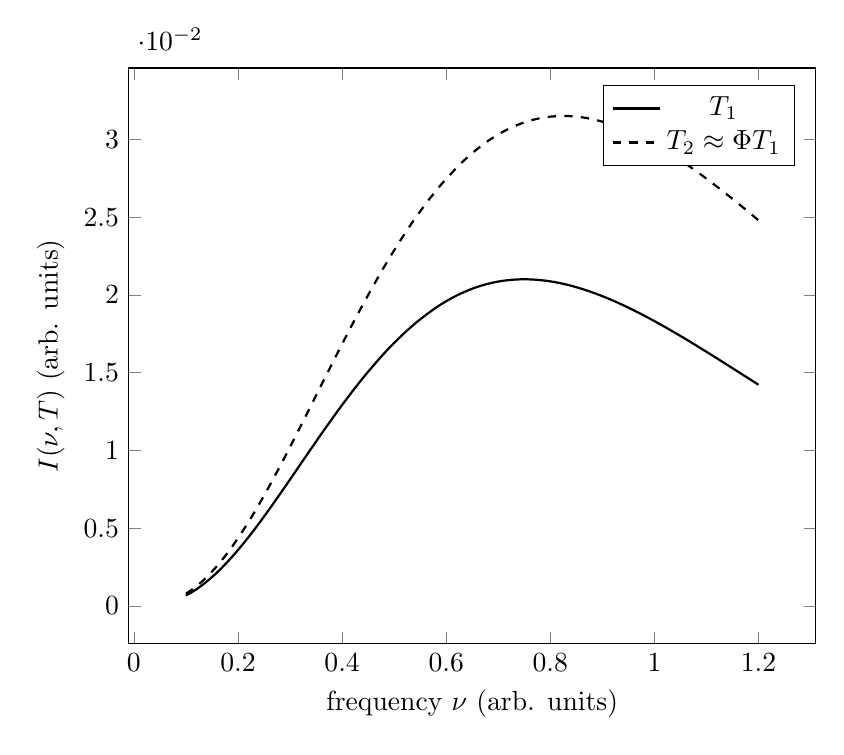
\begin{tikzpicture}
		\begin{axis}[
			width=0.85\textwidth,
			xlabel={frequency $\nu$ (arb. units)},
			ylabel={$I(\nu,T)$ (arb. units)},
			legend style={at={(0.97,0.97)},anchor=north east},
			domain=0.1:1.2,
			]
			
			% first illustrative spectrum (T1)
			\addplot[thick, samples=100] 
			{x^3 * exp(-4*x)};
			\addlegendentry{$T_1$};
			
			% second illustrative spectrum (T2 = Phi * T1) as shifted and scaled
			\addplot[thick, dashed, samples=100] 
			{1.5 * (x/1.1)^3 * exp(-4*(x/1.1))};
			\addlegendentry{$T_2 \approx \Phi T_1$};
			
		\end{axis}
	\end{tikzpicture}
	\caption{Illustrative black--body--like spectra at two temperatures $T_1$ and 
		$T_2 \approx \Phi T_1$. The curves are schematic but emphasize how the peak and 
		shape scale with temperature, consistent with the $\Phi$--geometric interpretation.}
	\label{fig:bb_spectra_phi}
\end{figure}

\begin{figure}[h!]
	\centering
	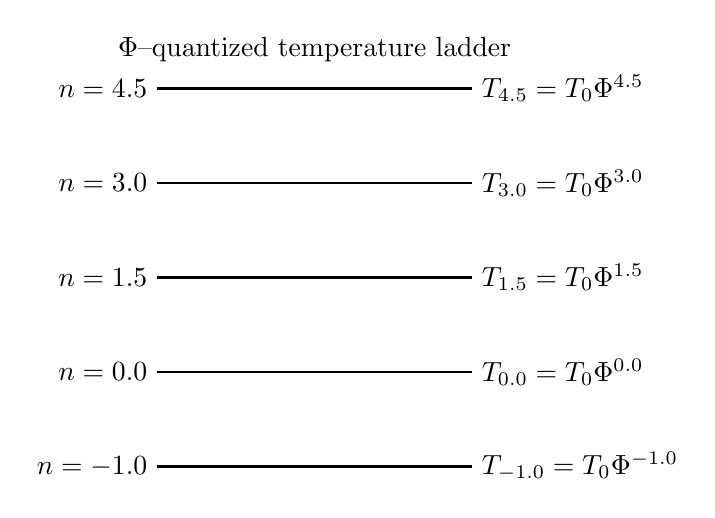
\begin{tikzpicture}[scale=1.0]
		
		% Ladder levels: n / y-coordinate
		\foreach \n/\y in {-1.0/0, 0.0/1.2, 1.5/2.4, 3.0/3.6, 4.5/4.8} {
			\draw[thick] (0,\y) -- (4,\y);
			\node[left]  at (0,\y) {$n=\n$};
			\node[right] at (4,\y) {$T_{\n} = T_0 \Phi^{\n}$};
		}
		
		\node at (2,5.3) {$\Phi$--quantized temperature ladder};
		
	\end{tikzpicture}
	\caption{Schematic $\Phi$--ladder of temperatures 
		$T_n = T_0 \Phi^n$, emphasising the geometric spacing of thermal scales and their
		direct mapping to frequencies via $f_n = (k_B/h) T_n$.}
	\label{fig:phi_temp_ladder}
\end{figure}

\begin{figure}[h!]
	\centering
	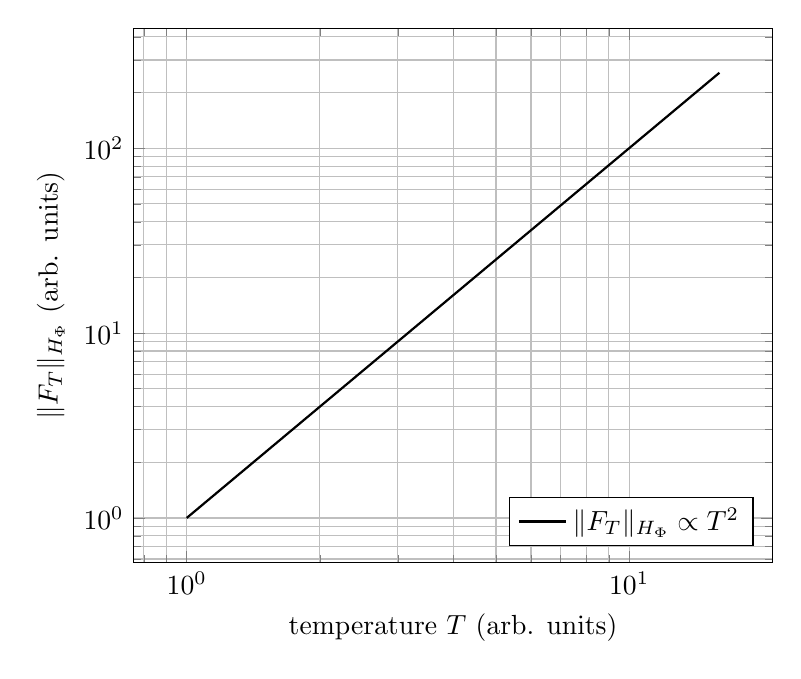
\begin{tikzpicture}
		\begin{axis}[
			width=0.8\textwidth,
			xmode=log,
			ymode=log,
			xlabel={temperature $T$ (arb. units)},
			ylabel={$\|F_T\|_{H_\Phi}$ (arb. units)},
			legend style={at={(0.97,0.03)},anchor=south east},
			grid=both,
			]
			
			% illustrative data following ||F_T|| ~ T^2
			\addplot[thick] coordinates {
				(1,   1)
				(2,   4)
				(4,   16)
				(8,   64)
				(16,  256)
			};
			
			\addlegendentry{$\|F_T\|_{H_\Phi} \propto T^2$};
			
		\end{axis}
	\end{tikzpicture}
	\caption{Log--log plot of the Hilbert--space norm $\|F_T\|_{H_\Phi}$ versus temperature $T$,
		illustrating the relation $\|F_T\|_{H_\Phi} \propto T^2$, which follows from 
		$P(T) \propto \|F_T\|_{H_\Phi}^2 \propto T^4$.}
	\label{fig:hilbert_vs_T}
\end{figure}


\begin{figure}[h!]
	\centering
	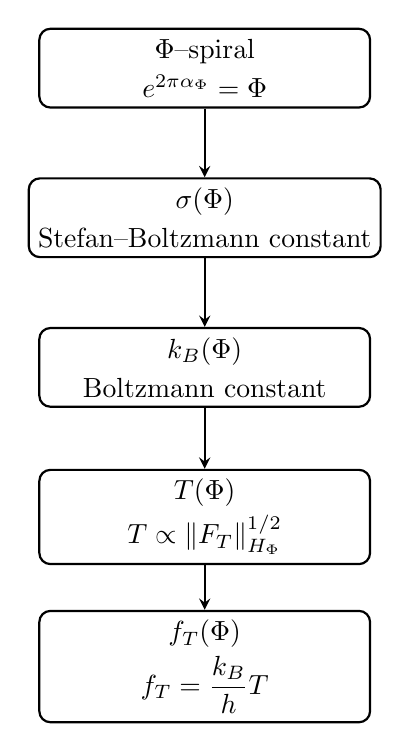
\begin{tikzpicture}[node distance=1.9cm, >=stealth, thick]
		
		% Styles
		\tikzstyle{block} = [draw, rounded corners, align=center, minimum width=4.2cm, minimum height=1cm];
		
		% Nodes
		\node[block] (phi) 
		{$\Phi$--spiral\\[2pt] $e^{2\pi\alpha_\Phi}=\Phi$};
		
		\node[block, below of=phi] (sigma)
		{$\sigma(\Phi)$\\[2pt] Stefan--Boltzmann constant};
		
		\node[block, below of=sigma] (kb)
		{$k_B(\Phi)$\\[2pt] Boltzmann constant};
		
		\node[block, below of=kb] (T)
		{$T(\Phi)$\\[2pt] $T \propto \|F_T\|_{H_\Phi}^{1/2}$};
		
		\node[block, below of=T] (fT)
		{$f_T(\Phi)$\\[2pt] $f_T = \dfrac{k_B}{h} T$};
		
		% Arrows
		\draw[->] (phi) -- (sigma);
		\draw[->] (sigma) -- (kb);
		\draw[->] (kb) -- (T);
		\draw[->] (T) -- (fT);
		
	\end{tikzpicture}
	
	\caption{Geometric flow diagram:
		$\Phi$--spiral $\rightarrow \sigma(\Phi) \rightarrow k_B(\Phi) \rightarrow T(\Phi) \rightarrow f_T(\Phi)$.
		Each quantity inherits its scaling from the logarithmic spiral identity.}
	\label{fig:phi_flow_chain}
\end{figure}

\section*{Acknowledgment}

I thank ChatGPT for assistance in structuring, formatting and great revision of the manuscript.

\begin{thebibliography}{99}
	
	\bibitem{Planck1901}
	M.~Planck,
	\textit{On the Law of Distribution of Energy in the Normal Spectrum},
	Annalen der Physik, 1901.
	
	\bibitem{Boltzmann1896}
	L.~Boltzmann,
	\textit{Vorlesungen über Gastheorie},
	1896.
	
	\bibitem{Stefan1879}
	J.~Stefan,
	\textit{Über die Beziehung zwischen der Wärmestrahlung und der Temperatur},
	Sitzungsberichte der Kaiserlichen Akademie der Wissenschaften, 1879.
	
	\bibitem{Hawking1975}
	S.~Hawking,
	\textit{Particle Creation by Black Holes},
	Communications in Mathematical Physics, 43 (1975), 199–220.
	
	\bibitem{BE1924}
	S.~Bose,
	\textit{Planck’s Law and the Hypothesis of Light Quanta},
	Zeitschrift für Physik, 1924.
	
	\bibitem{Einstein1925}
	A.~Einstein,
	\textit{Quantum Theory of the Monatomic Ideal Gas},
	Sitzungsberichte, Preussische Akademie der Wissenschaften, 1925.
	
	\bibitem{Riemann1859}
	B.~Riemann,
	\textit{Über die Anzahl der Primzahlen unter einer gegebenen Größe},
	Monatsberichte der Berliner Akademie, 1859.
	
	\bibitem{ZetaBE}
	N.~D. Mermin,
	\textit{Bose–Einstein condensation and the Riemann zeta function},
	American Journal of Physics, 1975.
	
	\bibitem{GammaFunction}
	E.~Whittaker and G.~Watson,
	\textit{A Course of Modern Analysis},
	Cambridge University Press.
	
	\bibitem{Kolarec_Phi_2025}
	R.~Kolarec,
	\textit{The Golden Ratio as the Universal Geometric Invariant: A Group-Theoretic Characterization via Spiral Symmetries},
	Zenodo (2025).
	\href{https://doi.org/10.5281/zenodo.17516329}{doi:10.5281/zenodo.17516329}.
	
	\bibitem{Kolarec_ComplexPlane_2025}
	R.~Kolarec,
	\textit{$\Phi$–Real Reparametrization of the Complex Plane and the Axiomatization of the $\varphi$–Fourier Transform },
	Zenodo (2025).
	\href{https://doi.org/10.5281/zenodo.17502838}{doi:10.5281/zenodo.17502838}.
	
	\bibitem{Kolarec_UGRC_2025}
	R.~Kolarec,
	\textit{The Universal Golden Resonance Constant (UGRC): Kolarec--Planck Ladder and the Exponential $\varphi$--Damping Kernel},
	Zenodo (2025).
	\href{https://doi.org/10.5281/zenodo.17459606}{doi:10.5281/zenodo.17459606}.
	
	\bibitem{Kolarec_Euler}
	R.~Kolarec,
	\textit{Euler Number e as the Exponential Kernel of the Golden Ratio Spiral},
	Zenodo (2025).
	\href{https://doi.org/10.5281/zenodo.17561612}{doi:10.5281/zenodo.17561612}.
	
	\bibitem{Kolarec_Superconduct_2025}
	R.~Kolarec,
	\textit{$\Phi$--Quantization of Superconducting Critical Temperatures},
	Zenodo (2025).
	\href{https://doi.org/10.5281/zenodo.17486930}{doi:10.5281/zenodo.17486930}.
	
	\bibitem{Kolarec2025_Fourier}
	R.~Kolarec,
	\textit{Axiomatization of $\Phi$--Fourier Analysis and an Exponential Convergence Theorem},
	Zenodo (2025).
	\href{https://doi.org/10.5281/zenodo.17451104}{doi:10.5281/zenodo.17451104}.
	
	\bibitem{Kolarec2025_Multilogy}
	R.~Kolarec,
	\textit{$\Phi$--Unified Resonant Multilogy: Master Framework},
	Zenodo (2025).
	\href{https://doi.org/10.5281/zenodo.17489221}{doi:10.5281/zenodo.17489221}.
	
	\bibitem{Kolarec2025_MB}
	R.~Kolarec,
	\textit{The $\Phi$--Maxwell--Boltzmann Distribution and Resonant Operator Framework},
	Zenodo (2025).
	\href{https://doi.org/10.5281/zenodo.17560639}{doi:10.5281/zenodo.17560639}.
	
	\bibitem{Kolarec2025_Orbit}
	R.~Kolarec,
	\textit{$\Phi$--Quantized Orbital Mechanics: Three–Body and N–Body Resonant Lattices on a Two–Sided Phi–Frequency Grid},
	Zenodo (2025).
	\href{https://doi.org/10.5281/zenodo.17460617}{doi:10.5281/zenodo.17460617}.

	\bibitem{Kolarec2025_Planck}
	R.~Kolarec,
	\textit{$Phi$–Resonant Architecture of Planetary Systems and Conscious Coupling: The Kolarec–Planck Framework on a Two–Sided Phi–Frequency Grid},
	Zenodo (2025).
	\href{ https://doi.org/10.5281/zenodo.17469444}{doi:10.5281/zenodo.17469444}.
	
\end{thebibliography}
\end{document}